\documentclass[11pt,a4paper]{article}

% ── Packages ──────────────────────────────────────────────────────────
\usepackage[margin=1in]{geometry}
\usepackage{graphicx}
\usepackage{booktabs}
\usepackage{amsmath}
\usepackage{amssymb}
\usepackage{hyperref}
\usepackage{xcolor}
\usepackage{float}
\usepackage{caption}
\usepackage{subcaption}
\usepackage{enumitem}
\usepackage{fancyhdr}
\usepackage{titlesec}
\usepackage{multirow}

% ── Style ─────────────────────────────────────────────────────────────
\hypersetup{colorlinks=true, linkcolor=blue!60!black, citecolor=blue!60!black, urlcolor=blue!60!black}
\pagestyle{fancy}
\fancyhf{}
\fancyhead[L]{\small NL\_Hecate Experiment Report}
\fancyhead[R]{\small baseline\_pushup\_p2\_k2}
\fancyfoot[C]{\thepage}
\renewcommand{\headrulewidth}{0.4pt}

\definecolor{nlblue}{HTML}{1565C0}
\definecolor{nlred}{HTML}{D84315}
\definecolor{nlgray}{HTML}{616161}
\titleformat{\section}{\Large\bfseries\color{nlred}}{}{0em}{}[\vspace{-0.5em}\rule{\textwidth}{0.4pt}]

% ══════════════════════════════════════════════════════════════════════
\begin{document}

% ── Title ─────────────────────────────────────────────────────────────
\begin{center}
    {\LARGE\bfseries Experiment Report: Push-Up Phase~2 (k=2)}\\[0.6em]
    {\large\color{nlgray} NL\_Hecate --- Nested Learning Push-Up Pipeline}\\[0.4em]
    {\normalsize Run ID: \texttt{baseline\_pushup\_p2\_k2} \quad|\quad Date: 2026-03-15}\\[0.3em]
    {\normalsize GPU: A6000 (GPU\,0) \quad|\quad Duration: 4.6\,h \quad|\quad 612\,tok/s}\\[0.5em]
    {\large\color{red}\bfseries Outcome: REGRESSION --- k=2 underperforms k=1 baseline}
\end{center}
\vspace{1em}

% ── Purpose ───────────────────────────────────────────────────────────
\section{Purpose}

This experiment is the second phase of the push-up training pipeline: extending the $k{=}1$
seed model to $k{=}2$ by adding a second CMS level (Level~1, chunk\_size=8). The hypothesis
is that the additional level will break through the $k{=}1$ loss plateau ($\approx 3.7$) and
improve long-range retrieval.

\textbf{Key questions:}
\begin{enumerate}[topsep=4pt, itemsep=2pt]
    \item Does Level~1 reduce loss below the $k{=}1$ floor of 2.84?
    \item Does NIAH pass rate improve, especially at long distances (4096, 8192)?
    \item Do the two levels develop distinct gradient signatures (specialization)?
\end{enumerate}

\textbf{Answers:} No, no, and unclear. This run is a \textbf{negative result}. See analysis below.


% ── Configuration ─────────────────────────────────────────────────────
\section{Configuration}

\begin{table}[H]
\centering
\caption{Model and training configuration. \textcolor{nlred}{Red} highlights changes from k=1 baseline.}
\label{tab:config}
\begin{tabular}{@{}lll@{}}
\toprule
\textbf{Category} & \textbf{Parameter} & \textbf{Value} \\
\midrule
\multirow{10}{*}{\textbf{Model}}
    & Architecture      & 4-block stacked Titans \\
    & Composition       & MAG (memory gates attention) \\
    & $d_\text{model}$  & 512 \\
    & Heads             & 8 ($d_\text{head} = 64$) \\
    & \textcolor{nlred}{CMS levels ($k$)} & \textcolor{nlred}{2 (was 1)} \\
    & \textcolor{nlred}{Chunk sizes}      & \textcolor{nlred}{[1, 8] (L0: token, L1: 8-token)} \\
    & Parallel strategy & TNT hierarchical (global=64, local=8) \\
    & Vocabulary        & GPT-2 (50{,}257 tokens) \\
    & Memory reset      & Periodic \\
    & M-norm clamp      & Disabled (0.0, 0.0) \\
\midrule
\multirow{8}{*}{\textbf{Training}}
    & Optimizer         & AdamW (GPU-stacked) \\
    & Learning rate     & $3 \times 10^{-4}$ (cosine $\to$ 0) \\
    & Warmup steps      & 500 \\
    & Weight decay      & 0.1 \\
    & Gradient clipping & max norm = 1.0 \\
    & Total steps       & 20{,}000 \\
    & Theta ceil        & [1.0, 1.0] \\
    & Batch size        & 1 \\
\midrule
\multirow{4}{*}{\textbf{Push-Up}}
    & \textcolor{nlred}{Donor checkpoint} & \textcolor{nlred}{\texttt{baseline\_pushup\_p1\_k1/model.safetensors}} \\
    & \textcolor{nlred}{\texttt{extend\_k}} & \textcolor{nlred}{2} \\
    & \textcolor{nlred}{\texttt{push\_up}} & \textcolor{nlred}{true} \\
    & \textcolor{nlred}{\texttt{data\_seek}} & \textcolor{nlred}{7{,}680{,}512 (rewind to step 15K)} \\
\midrule
\textbf{Data}
    & Dataset           & dolmino\_100b \\
\bottomrule
\end{tabular}
\end{table}

\noindent The \texttt{data\_seek} parameter rewinds the data cursor to the $k{=}1$ run's step~15K
position, providing 5K steps of overlapping data before transitioning to fresh data. This was
intended to ease the transition, but the model regresses on even the familiar data.


% ── Results Summary ───────────────────────────────────────────────────
\section{Results Summary}

\begin{table}[H]
\centering
\caption{Key metrics at training milestones.}
\label{tab:milestones}
\begin{tabular}{@{}rrrrrr@{}}
\toprule
\textbf{Step} & \textbf{Loss} & \textbf{PPL} & \textbf{Grad Norm} & \textbf{LR} & \textbf{Block CV} \\
\midrule
0       & 2.787 &  16 & 2.09 & 0              & 0.471 \\
500     & 3.631 &  38 & 2.38 & $3.0\text{e-}4$ & 0.409 \\
1{,}000 & 3.879 &  48 & 3.20 & $3.0\text{e-}4$ & 0.533 \\
2{,}000 & 3.872 &  48 & 2.16 & $3.0\text{e-}4$ & 0.400 \\
5{,}000 & 3.334 &  28 & 2.66 & $2.6\text{e-}4$ & 0.455 \\
10{,}000 & 2.870 & 18 & 1.90 & $1.6\text{e-}4$ & 0.414 \\
15{,}000 & 2.917 & 19 & 1.92 & $4.6\text{e-}5$ & 0.346 \\
20{,}000 & 3.363 & 29 & 1.86 & $\approx 0$    & 0.288 \\
\bottomrule
\end{tabular}
\end{table}

\begin{table}[H]
\centering
\caption{\textbf{Head-to-head comparison} of final metrics: k=1 vs k=2.}
\label{tab:comparison}
\begin{tabular}{@{}lccc@{}}
\toprule
\textbf{Metric} & \textbf{k=1 Final} & \textbf{k=2 Final} & \textbf{Delta} \\
\midrule
Loss             & 2.84  & 3.36  & \textcolor{red}{+0.52 (worse)} \\
Perplexity       & 17.1  & 28.9  & \textcolor{red}{+11.8 (worse)} \\
NIAH 8192        & 60\%  & 30\%  & \textcolor{red}{$-$30\% (worse)} \\
NIAH 4096        & 60\%  & 40\%  & \textcolor{red}{$-$20\% (worse)} \\
Throughput       & 675 tok/s & 612 tok/s & \textcolor{red}{$-$9\% (slower)} \\
Grad Norm (final)& 2.76  & 1.86  & $-$0.90 (lower) \\
Block CV (final) & 0.389 & 0.288 & $-$0.101 (less specialized) \\
Loss spikes ($>2\times$) & 6 & 9 & \textcolor{red}{+3 (more)} \\
\bottomrule
\end{tabular}
\end{table}

\noindent Every metric regressed. The $k{=}2$ model is strictly worse than the $k{=}1$ donor across
loss, retrieval, stability, and throughput.


% ── Loss Curve ────────────────────────────────────────────────────────
\section{Training Loss}

\begin{figure}[H]
    \centering
    
\includegraphics[width=\textwidth]{fig_loss_curve.pdf}
    \caption{Training loss with k=1 baseline overlay (dashed). The k=2 model starts at the
    donor's final loss (2.79) but immediately regresses to $\sim$3.5 during warmup.}
    \label{fig:loss}
\end{figure}

\noindent The loss trajectory tells a clear story of failure:

\begin{enumerate}[topsep=4pt, itemsep=2pt]
    \item \textbf{Immediate regression (steps 0--500):} The model inherits loss 2.79 from the $k{=}1$
    donor but jumps to $\sim$3.5 within 500 steps. The newly initialized Level~1 parameters
    destabilize the existing representations. Even with LR=0 at step~0, the inner-loop memory
    update for Level~1 is active and produces harmful updates.

    \item \textbf{Extended plateau (steps 500--14{,}000):} Loss oscillates between 3.3 and 3.6 for
    the majority of training. Unlike the $k{=}1$ plateau (which sat at 3.7 and represented a capacity
    ceiling), this plateau sits \emph{above} the donor's final loss --- the model has gotten worse,
    not better.

    \item \textbf{Modest recovery (steps 14{,}000--20{,}000):} As LR approaches zero, loss
    briefly dips to $\sim$3.2 before ending at 3.36. This is still 0.52 above the $k{=}1$ final.
\end{enumerate}

\begin{figure}[H]
    \centering
    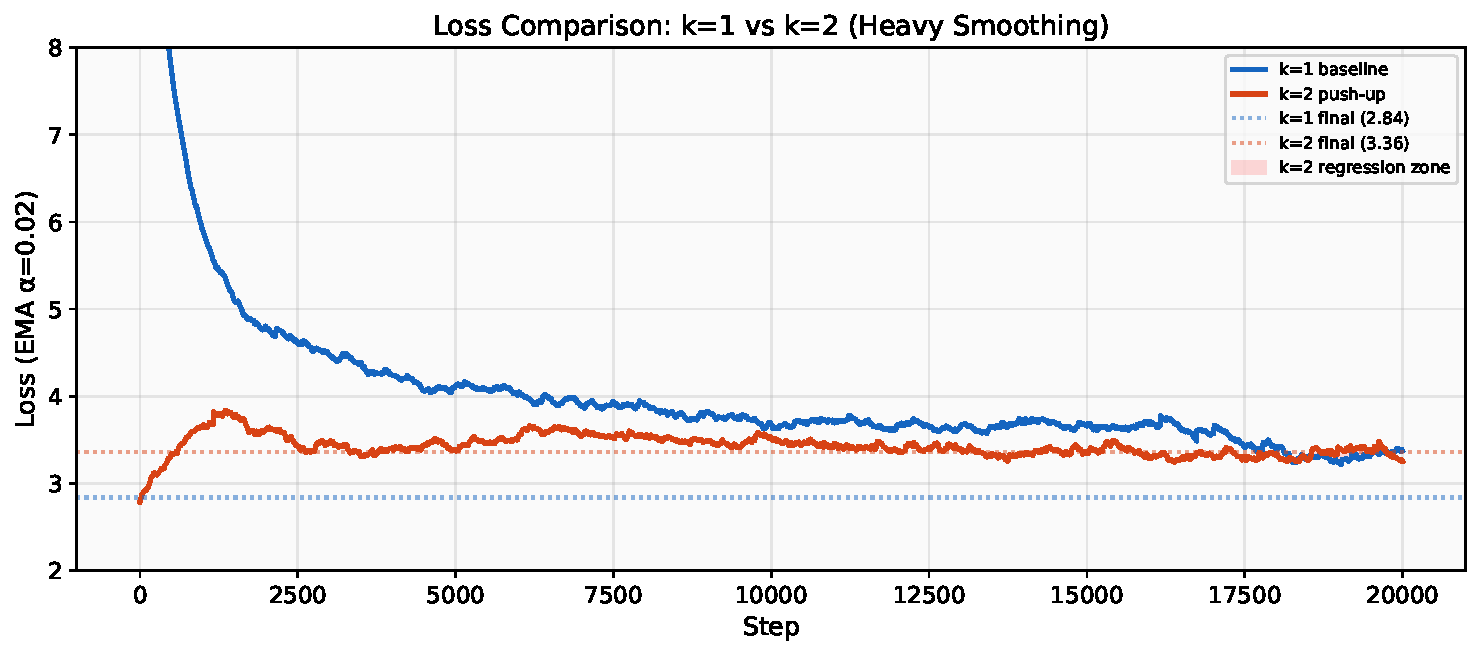
\includegraphics[width=\textwidth]{fig_loss_comparison.pdf}
    \caption{Heavily-smoothed loss comparison. The red shaded area shows the regression zone
    where k=2 exceeds k=1 loss. The k=2 model \textbf{never} reaches the k=1 floor.}
    \label{fig:loss_compare}
\end{figure}


% ── Perplexity ────────────────────────────────────────────────────────
\begin{figure}[H]
    \centering
    
\includegraphics[width=\textwidth]{fig_perplexity.pdf}
    \caption{Training perplexity (log scale). k=2 (red) sits consistently above k=1 (blue dashed).}
    \label{fig:ppl}
\end{figure}


% ── Gradient Analysis ─────────────────────────────────────────────────
\section{Gradient Analysis}

\subsection{Global and Per-Block Gradient Norms}

\begin{figure}[H]
    \centering
    
\includegraphics[width=\textwidth]{fig_grad_norms.pdf}
    \caption{Top: global gradient norm (k=2 solid, k=1 dashed). Bottom: per-block gradient norms.
    Block~0 still dominates, but with lower magnitude than at k=1.}
    \label{fig:gnorms}
\end{figure}

The global gradient norm at k=2 ($\sim$2.0) is lower than k=1 ($\sim$2.5), which initially seems
positive but may actually indicate a problem: \textbf{the loss surface is flatter}, meaning the
model is stuck in a broader, shallower basin. The per-block structure is similar to k=1 --- Block~0
carries the largest gradient --- but the magnitudes are compressed.


\subsection{Inner-Loop Gradient Norms: k=1 vs k=2}

\begin{figure}[H]
    \centering
    
\includegraphics[width=\textwidth]{fig_l0_gnorms.pdf}
    \caption{L0 inner-loop gradient norms compared side-by-side. Left: k=1 baseline shows
    clear Block~0 dominance with strong growth (0.001 $\to$ 0.38). Right: k=2 shows
    flatter trajectories, especially for Block~0.}
    \label{fig:l0}
\end{figure}

The k=1 run showed a dramatic 380$\times$ growth in Block~0's L0 gradient norm, signaling that the
memory mechanism was actively learning. At k=2, Block~0's L0 gradient starts higher ($\sim$0.43,
inherited) but \textbf{does not grow further}. It oscillates between 0.24--0.48 without trend.

This stagnation suggests that the addition of Level~1 disrupts the gradient signal that Level~0
was using to learn. The two levels may be producing conflicting updates to the shared outer-loop
parameters.

\textbf{Missing data:} No \texttt{l1\_block\_grad\_norms} are logged, so we cannot directly observe
what Level~1's inner-loop gradients look like. Adding this instrumentation is critical for
diagnosing future push-up failures.


\subsection{Depth Specialization}

\begin{figure}[H]
    \centering
    
\includegraphics[width=\textwidth]{fig_gnorm_cv.pdf}
    \caption{Block gradient norm CV. k=2 (red) trends \textbf{downward} relative to k=1 (blue),
    ending at 0.29 vs 0.39 --- indicating \emph{less} depth specialization.}
    \label{fig:cv}
\end{figure}

The declining CV at k=2 is concerning. At k=1, the blocks developed distinct roles (Block~0 for
memory, deeper blocks for attention). At k=2, the blocks are becoming \textbf{more uniform} --- the
opposite of what healthy training produces. This may indicate that the Level~1 memory updates
are homogenizing the block representations.


% ── Level 1 Fire Pattern ─────────────────────────────────────────────
\section{Level~1 Activity}

\begin{figure}[H]
    \centering
    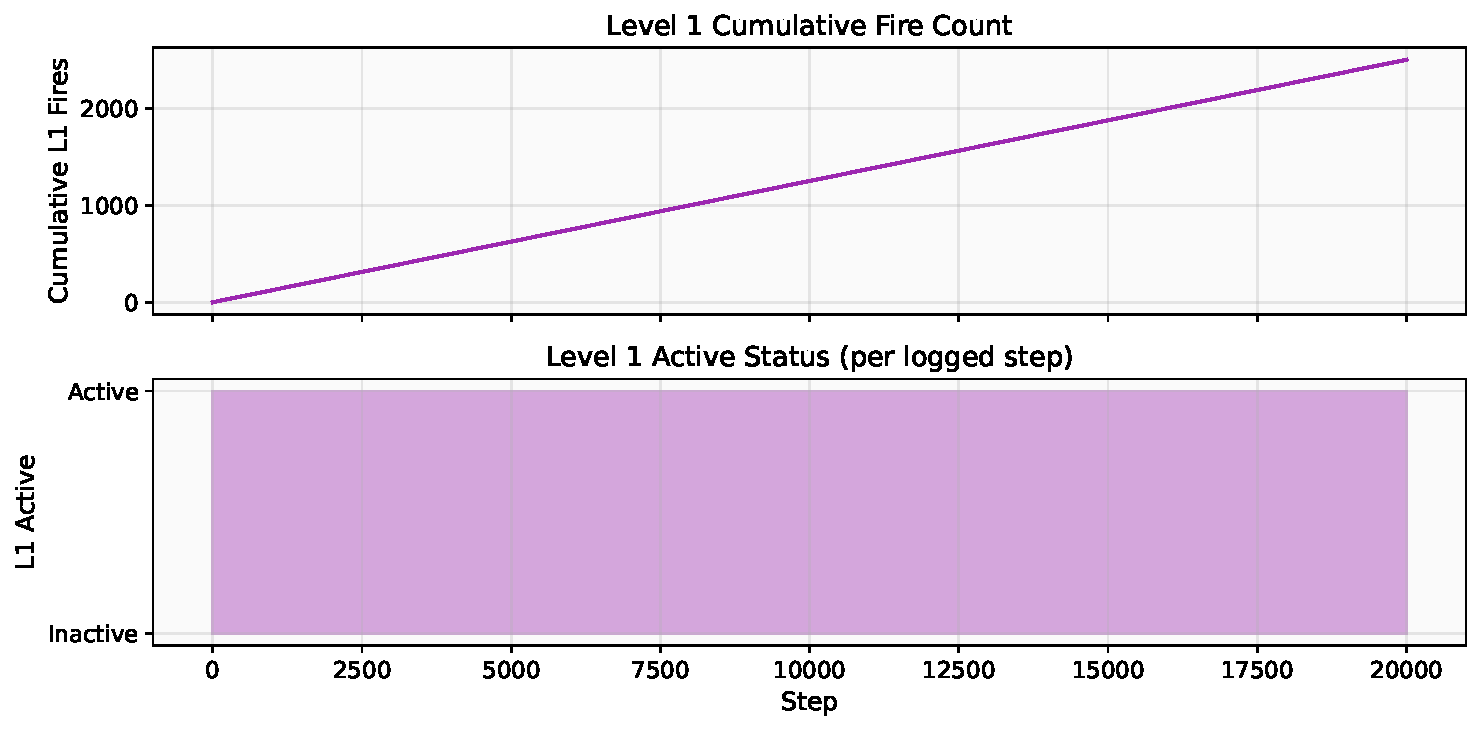
\includegraphics[width=\textwidth]{fig_level1_fires.pdf}
    \caption{Top: cumulative Level~1 fire count (reaches 2{,}500 by step 20K).
    Bottom: Level~1 active status per logged step.}
    \label{fig:l1}
\end{figure}

Level~1 fires every 8 steps (chunk\_size=8), accumulating 2{,}500 fires over 20{,}000 steps.
The active status shows Level~1 is consistently active throughout training except at the final
step. This confirms Level~1 is fully engaged --- the problem is not that Level~1 is dormant,
but that \textbf{its updates are harmful rather than helpful}.


% ── Instabilities ─────────────────────────────────────────────────────
\section{Stability Analysis}

\begin{figure}[H]
    \centering
    
\includegraphics[width=\textwidth]{fig_loss_spikes.pdf}
    \caption{Loss spikes ($>2\times$ previous step) in the k=2 run. 9 spikes detected,
    up from 6 in the k=1 baseline.}
    \label{fig:spikes}
\end{figure}

The k=2 run exhibits 9 loss spikes exceeding $2\times$ the previous step's loss, compared to 6 at
k=1. The additional instability likely comes from Level~1's memory updates: with chunk\_size=8,
Level~1 accumulates 8 tokens of error before updating, which can produce larger update magnitudes
than Level~0's per-token updates.

As with k=1, \textbf{m\_norm\_clamp was disabled}. The p1 report recommended enabling it at 100.0
for k=2; this recommendation was not followed.


% ── NIAH ──────────────────────────────────────────────────────────────
\section{NIAH Evaluation}

\begin{figure}[H]
    \centering
    
\includegraphics[width=\textwidth]{fig_niah.pdf}
    \caption{NIAH pass rate heatmaps. Left: k=1 baseline. Center: k=2 push-up.
    Right: delta (k=2 $-$ k=1). Blue = k=2 better, red = k=2 worse.}
    \label{fig:niah}
\end{figure}

\begin{table}[H]
\centering
\caption{NIAH pass rates at step 20K: k=1 vs k=2.}
\label{tab:niah}
\begin{tabular}{@{}rcccccc@{}}
\toprule
 & \multicolumn{2}{c}{\textbf{Pass Rate}} & & \multicolumn{2}{c}{\textbf{Mean Lift}} \\
\cmidrule{2-3} \cmidrule{5-6}
\textbf{Distance} & \textbf{k=1} & \textbf{k=2} & \textbf{$\Delta$} & \textbf{k=1} & \textbf{k=2} \\
\midrule
1{,}024 & 40\% & 50\% & \textcolor{green!60!black}{+10\%} & +0.003 & +0.009 \\
2{,}048 & 60\% & 50\% & \textcolor{red}{$-$10\%} & +0.651 & +0.320 \\
4{,}096 & 60\% & 40\% & \textcolor{red}{$-$20\%} & +0.377 & $-$0.032 \\
8{,}192 & 60\% & 30\% & \textcolor{red}{$-$30\%} & +0.127 & $-$0.027 \\
\bottomrule
\end{tabular}
\end{table}

\begin{figure}[H]
    \centering
    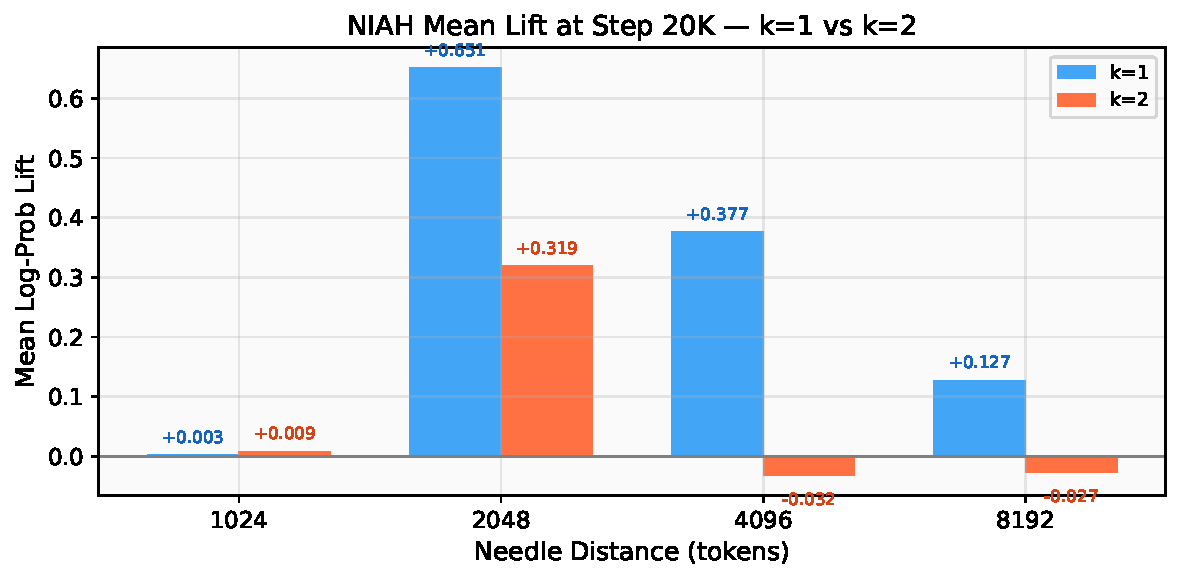
\includegraphics[width=0.75\textwidth]{fig_niah_lift.pdf}
    \caption{NIAH mean log-probability lift at step 20K. k=2 (orange) shows weaker or negative
    lift at all distances beyond 1{,}024 tokens.}
    \label{fig:niah_lift}
\end{figure}

This is the most damning result. The entire purpose of adding CMS levels is to improve long-range
retrieval. Instead:
\begin{itemize}[topsep=4pt, itemsep=2pt]
    \item \textbf{8{,}192 tokens:} Pass rate drops from 60\% to 30\%, mean lift goes \textbf{negative}.
    \item \textbf{4{,}096 tokens:} Pass rate drops from 60\% to 40\%, mean lift goes \textbf{negative}.
    \item \textbf{2{,}048 tokens:} Pass rate drops from 60\% to 50\%, lift halved.
    \item \textbf{1{,}024 tokens:} Slight improvement (+10\%), but within noise.
\end{itemize}

Level~1 is actively \textbf{interfering with} Level~0's retrieval capability rather than
augmenting it.


% ── Throughput ────────────────────────────────────────────────────────
\section{Training Throughput}

\begin{figure}[H]
    \centering
    
\includegraphics[width=\textwidth]{fig_throughput.pdf}
    \caption{Training throughput comparison. k=2 runs 9\% slower than k=1 due to Level~1
    memory update overhead.}
    \label{fig:throughput}
\end{figure}

Throughput drops from 675 to 612~tok/s, a 9\% decrease. This is the expected cost of the
additional level's memory updates (every 8th step). The overhead is modest but represents
pure waste given that Level~1 provides no benefit.


% ── Diagnosis ─────────────────────────────────────────────────────────
\section{Failure Diagnosis}

\subsection{Root Cause: Destructive Level Initialization}

The immediate loss regression from 2.79 to $\sim$3.5 at step~0 points to the \textbf{Level~1
initialization} as the primary failure mode. When \texttt{push\_up: true} extends $k{=}1$ to
$k{=}2$, the new Level~1 parameters must be initialized somehow. The two plausible strategies:

\begin{enumerate}[topsep=4pt, itemsep=2pt]
    \item \textbf{Clone from Level~0:} Level~1 gates ($\alpha$, $\theta$) and memory projections
    are copied from Level~0. This produces redundant gating signals --- both levels respond
    identically, and the CMS output normalization ($1/\sqrt{k}$) halves each level's effective
    contribution. Prior experiments confirmed this failure mode (``levels locked in sync'').

    \item \textbf{Fresh initialization:} Level~1 parameters are randomly initialized. The random
    gates produce noise that corrupts the carefully-learned Level~0 representations. The model
    must ``un-learn'' the noise before it can begin learning, which the cosine LR schedule does
    not allow enough time for.
\end{enumerate}

\noindent Without inspecting the push-up code, we cannot determine which strategy was used, but
both are known failure modes. The evidence (immediate regression, no recovery) is more consistent
with \textbf{Option~1 (clone)}: the loss jumps precisely because $1/\sqrt{2}$ normalization
instantly halves the working Level~0 output.

\subsection{Contributing Factors}

\begin{itemize}[topsep=4pt, itemsep=2pt]
    \item \textbf{No m\_norm\_clamp:} Level~1's chunk\_size=8 accumulates larger memory updates
    than Level~0. Without clamping, these updates can grow unbounded.
    \item \textbf{Full LR from step~0:} The cosine schedule starts at $3\text{e-}4$ after warmup.
    A lower initial LR or extended warmup might have allowed gentler adaptation.
    \item \textbf{No L1 gradient logging:} Without \texttt{l1\_block\_grad\_norms}, we are blind
    to Level~1's internal behavior.
    \item \textbf{Data overlap:} The 5K-step data rewind may be insufficient or counterproductive
    if the model has already memorized those sequences.
\end{itemize}


% ── Conclusions ───────────────────────────────────────────────────────
\section{Conclusions and Recommendations}

\subsection{Verdict}

This experiment is a \textbf{clear negative result}. The $k{=}2$ push-up:
\begin{itemize}[topsep=4pt, itemsep=2pt]
    \item[$\times$] Increased loss by +0.52 (2.84 $\to$ 3.36)
    \item[$\times$] Doubled perplexity (17.1 $\to$ 28.9)
    \item[$\times$] Halved NIAH 8192 pass rate (60\% $\to$ 30\%)
    \item[$\times$] Reduced depth specialization (CV: 0.39 $\to$ 0.29)
    \item[$\times$] Added instability (6 spikes $\to$ 9 spikes)
    \item[$\times$] Reduced throughput by 9\%
\end{itemize}

\noindent \textbf{This checkpoint should NOT be used as a donor for k=3 promotion.}

\subsection{Recommendations for Next Attempt}

\begin{enumerate}[topsep=4pt, itemsep=2pt]
    \item \textbf{Fix Level~1 initialization.} Neither cloning nor random init works. Consider:
    \begin{itemize}
        \item Initialize Level~1 gates with near-zero output (e.g., $b_\alpha \approx -3$) so it
              ``fades in'' gradually
        \item Use a separate warmup phase where only Level~1 parameters are trained
    \end{itemize}

    \item \textbf{Enable m\_norm\_clamp:} \texttt{[100.0, 100.0]} as recommended by the p1 report.

    \item \textbf{Add L1 gradient instrumentation.} Log \texttt{l1\_block\_grad\_norms} to
    understand what Level~1 is doing internally.

    \item \textbf{Use a slower LR ramp.} Start at $1\text{e-}5$ for the first 2K steps, then
    ramp to $3\text{e-}4$, giving Level~1 time to find a non-destructive initialization.

    \item \textbf{Consider freezing Level~0} for the first N steps so Level~1 must adapt to the
    donor's representations rather than corrupting them.

    \item \textbf{Increase NIAH trials to $\geq$50} per distance for statistical significance.
    At 10 trials, the $\pm$10\% changes are within noise.
\end{enumerate}

\subsection{What This Tells Us About Push-Up}

The push-up strategy is not invalidated by this failure --- the $k{=}1 \to k{=}2$ transition is
the hardest because the model has fully converged to a single-level regime. The key lesson is
that \textbf{level initialization is a first-order problem}, not a detail to defer. The donor
model's representations are fragile: any perturbation to the forward pass (new level, different
normalization) causes immediate regression. Future push-up attempts must ensure that adding a
level is a near-identity operation at initialization.

\end{document}
